\documentclass[12pt]{article}


\usepackage{amssymb}
\usepackage{amsmath}
\usepackage{fullpage}
\usepackage{epsfig}
\usepackage{epstopdf}
\everymath{\displaystyle}



\begin{document}

\begin{center}
\underline{\LARGE{Trigonometric Substitution}}
\end{center}

\noindent SUGGESTED REFERENCE MATERIAL:

\bigskip

\noindent As you work through the problems listed below, you should reference Chapter 7.4 of the recommended textbook (or the equivalent chapter in your alternative textbook/online resource) and your lecture notes.

\bigskip

\noindent EXPECTED SKILLS:

\begin{itemize}

\item Be able to evaluate integrals that involve particular expressions (see Table 7.4.1) by making the appropriate trigonometric substitution.

\item Know how to evaluate integrals that involve quadratic expressions by first completing the square and then making the appropriate substitution. 

\end{itemize}

\noindent PRACTICE PROBLEMS:

\medskip

\noindent{\bf For problems 1-12, evaluate the given integral.  Notice that it may not be necessary to use a trigonometric substitution for all problems.}

\begin{enumerate}

\item $\int \sqrt{3-x^2}\,dx$ 

\includegraphics[scale=0.5]{start.pdf}
{{$\frac{3}{2}\arcsin{\left(\frac{x}{\sqrt{3}}\right)}+\frac{1}{2}x\sqrt{3-x^2}+C$}}
\includegraphics[scale=0.5]{end.pdf}


\item $\int \frac{1}{(x^2+1)^2}\,dx$ 

\includegraphics[scale=0.5]{start.pdf}
{{$\frac{1}{2}\tan^{-1}{x}+\frac{x}{2(x^2+1)}+C$}}
\includegraphics[scale=0.5]{end.pdf}


\item $\int \frac{1}{\sqrt{4-x^2}}\,dx$ 

\includegraphics[scale=0.5]{start.pdf}
{{$\arcsin{\left(\frac{x}{2}\right)+C}$}}
\includegraphics[scale=0.5]{end.pdf}


\item $\int \frac{x}{\sqrt{1-4x^2}}\,dx$ 

\includegraphics[scale=0.5]{start.pdf}
{{$-\frac{1}{4}\sqrt{1-4x^2}+C$}}
\includegraphics[scale=0.5]{end.pdf}


\item $\int \frac{x^2}{\sqrt{1-2x^2}}\,dx$ 

\includegraphics[scale=0.5]{start.pdf}
{{$\frac{1}{4\sqrt{2}}\arcsin{(\sqrt{2}x)}-\frac{1}{4}x\sqrt{1-2x^2}+C$}}
\includegraphics[scale=0.5]{end.pdf}


\item $\int^{\sqrt{3}}_1 x\sqrt{x^2+1}\,dx$ 

\includegraphics[scale=0.5]{start.pdf}
{{$\frac{1}{3}(8-2\sqrt{2})$}}
\includegraphics[scale=0.5]{end.pdf}


\item $\int^2_{\sqrt{2}} \frac{\sqrt{4-x^2}}{x^2}\,dx$ 

\includegraphics[scale=0.5]{start.pdf}
{{$1-\frac{\pi}{4}$}}
\includegraphics[scale=0.5]{end.pdf}


\item $\int \frac{1}{x^2\sqrt{x^2+16}}\,dx$ 

\includegraphics[scale=0.5]{start.pdf}
{{$-\frac{\sqrt{x^2+16}}{16x}+C$}}
\includegraphics[scale=0.5]{end.pdf}


\item $\int_1^2 \frac{\sqrt{x^2-1}}{x}\,dx$ 

\includegraphics[scale=0.5]{start.pdf}
{{$\sqrt{3}-\frac{\pi}{3}$}}
\includegraphics[scale=0.5]{end.pdf}


\item $\int_{-\sqrt{5}}^{\sqrt{15}} \frac{1}{x^2+5}\,dx$ 

\includegraphics[scale=0.5]{start.pdf}
{{$\frac{7\pi}{12\sqrt{5}}$}}
\includegraphics[scale=0.5]{end.pdf}


\item $\int \frac{1}{4x^2-2x+17/4}\,dx$ 

\includegraphics[scale=0.5]{start.pdf}
{{$\frac{1}{4}\arctan{\left(x-\frac{1}{4}\right)}+C$}}
\includegraphics[scale=0.5]{end.pdf}


\item $\int \frac{1}{\sqrt{-x^2+4x-3}} \,dx$

\includegraphics[scale=0.5]{start.pdf}
{{$\sin^{-1}(x-2)+C$}}
\includegraphics[scale=0.5]{end.pdf}


\item Compute the area enclosed within the ellipse $\frac{x^2}{9}+\frac{y^2}{4}=1$.

\includegraphics[scale=0.5]{start.pdf}
{{$6\pi$}}
\includegraphics[scale=0.5]{end.pdf}


\item Let $R$ be the region in the $xy$-plane which is enclosed by $y=\frac{1}{x^2+1}$, $y=0$, $x=0$ and $x=1$.  Calculate the volume of the solid which results from revolving $R$ around the $x$-axis.  (Hint: see number 2 above.)

\includegraphics[scale=0.5]{start.pdf}
{{$\frac{\pi}{4}\left(\frac{\pi}{2}+1\right)$}}
\includegraphics[scale=0.5]{end.pdf}


\item Compute the length of the curve $y=x^2$ on the interval $\left[-\frac{\sqrt{3}}{2},\frac{1}{2}\right]$.  (Hint: See problem 25 (a) in the ``Trigonometric Integrals (Chapter 7.3)" homework.)

\includegraphics[scale=0.5]{start.pdf}
{{$\frac{\sqrt{2}}{4}+\frac{1}{4}\ln{\left|\sqrt{2}+1\right|}+\frac{\sqrt{3}}{2}-\frac{1}{4}\ln{\left|2-\sqrt{3}\right|}$}}
\includegraphics[scale=0.5]{end.pdf}


\item \begin{enumerate}

\item Evaluate $\int \frac{\sqrt{x^2+1}}{x} \,dx$.  (Hint: $\int \frac{\sec^3{\theta}}{\tan{\theta}} \,d\theta = \sec{\theta}-\ln{|\csc{\theta}+\cot{\theta}|}+C$)

\includegraphics[scale=0.5]{start.pdf}
{{$\sqrt{x^2+1}-\ln{\left|\frac{\sqrt{x^2+1}+1}{x}\right|}+C$}}
\includegraphics[scale=0.5]{end.pdf}


\item Compute the length of the curve $y=\ln{x}$ on the interval $[1,3]$.  (Hint: Use part a.)

\includegraphics[scale=0.5]{start.pdf}
{{$\sqrt{10}-\ln{\left(\frac{\sqrt{10}+1}{3}\right)}-\sqrt{2}+\ln{\left(\sqrt{2}+1\right)}$}}
\includegraphics[scale=0.5]{end.pdf}


\end{enumerate}

\item Consider the region $R$ which is enclosed by $y=\sqrt{4-x^2}$, $y=0$, $x=0$, and $x=1$, in the first quadrant.

\begin{center}
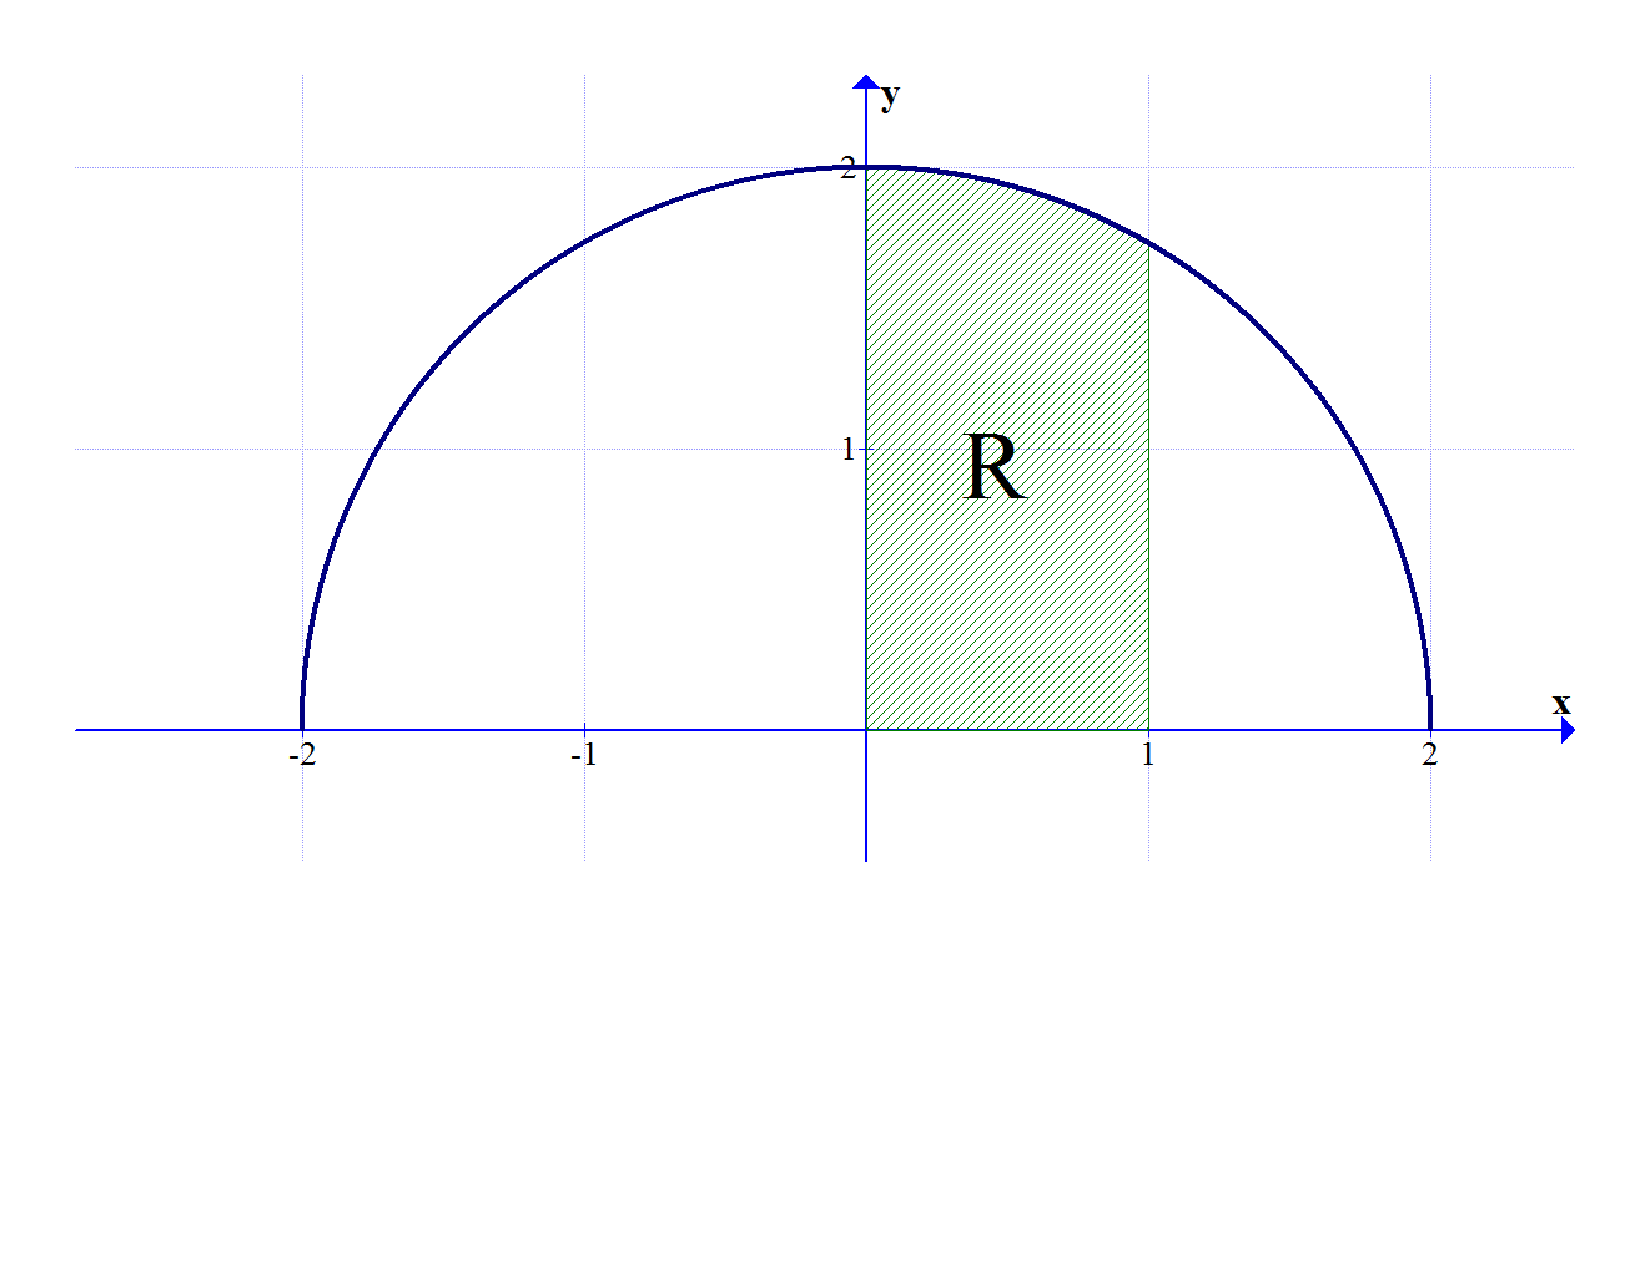
\includegraphics[scale=0.5]{area.pdf}
\end{center}

\begin{enumerate}

\item By evaluating an appropriate integral, compute the area of $R$.

\includegraphics[scale=0.5]{start.pdf}
{{$A=\int_0^1 \sqrt{4-x^2} \,dx=\frac{\pi}{3}+\frac{\sqrt{3}}{2}$}}
\includegraphics[scale=0.5]{end.pdf}


\item Verify your answer geometrially by combining the area of the sector and the area of the triangle, shown below.

\begin{center}
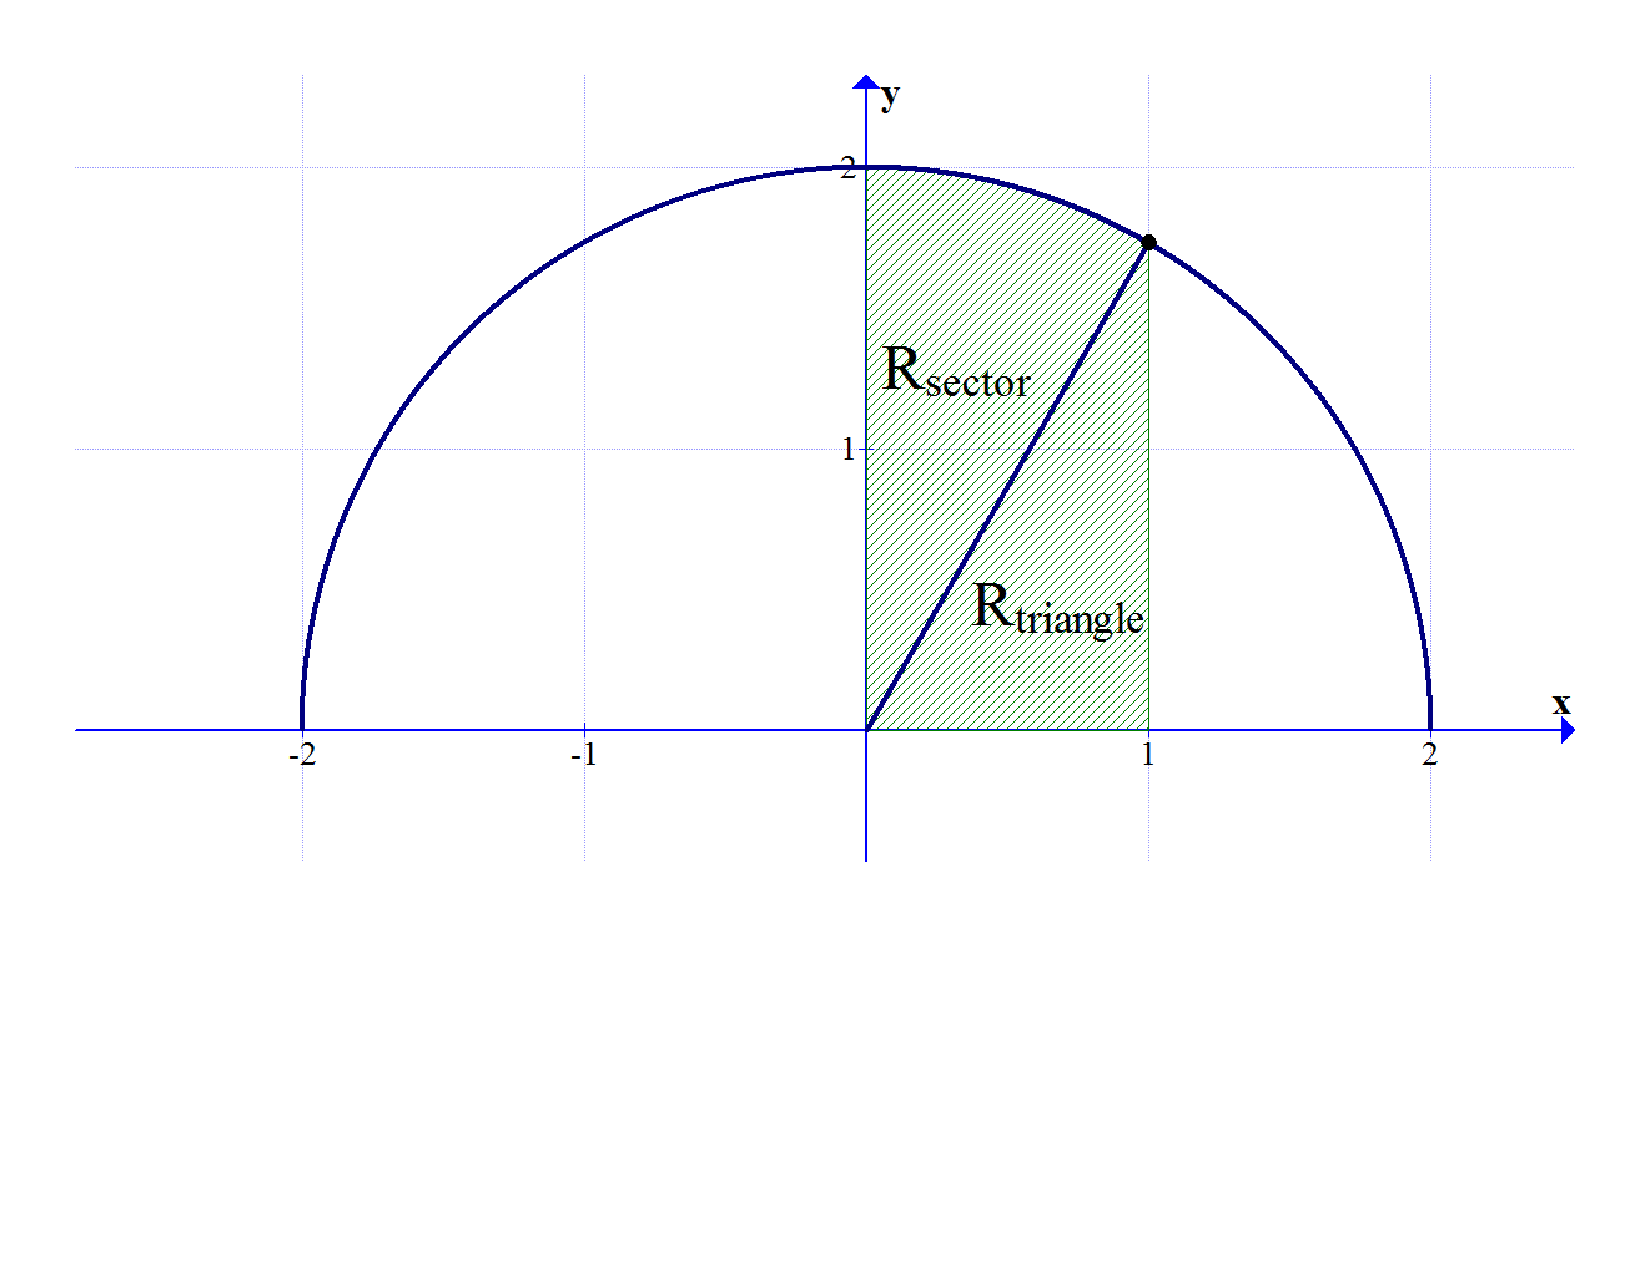
\includegraphics[scale=0.5]{area2.pdf}
\end{center}

\includegraphics[scale=0.5]{start.pdf}
{{$R_{\text{Triangle}}=\frac{1}{2}bh=\frac{1}{2}(1)\left(\sqrt{3}\right)=\frac{\sqrt{3}}{2}$; $R_{\text{Sector}}=\frac{1}{2}r^2\theta=\frac{1}{2}(2)^2\left(\frac{\pi}{6}\right)=\frac{\pi}{3}$}}
\includegraphics[scale=0.5]{end.pdf}


\end{enumerate}

\end{enumerate}

\end{document}